%%%%%%%%%%%%%%%%%%%%%%%%%%%%%%%%%%%%%%%%
% datoteka diploma-vzorec.tex
%
% vzorčna datoteka za pisanje diplomskega dela v formatu LaTeX
% na UL Fakulteti za računalništvo in informatiko
%
% vkup spravil Gašper Fijavž, december 2010
% 
%
%
% verzija 12. februar 2014 (besedilo teme, seznam kratic, popravki Gašper Fijavž)
% verzija 10. marec 2014 (redakcijski popravki Zoran Bosnić)
% verzija 11. marec 2014 (redakcijski popravki Gašper Fijavž)
% verzija 15. april 2014 (pdf/a 1b compliance, not really - just claiming, Damjan Cvetan, Gašper Fijavž)
% verzija 23. april 2014 (privzeto cc licenca)
% verzija 16. september 2014 (odmiki strain od roba)
% verzija 28. oktober 2014 (odstranil vpisno številko)
% verija 5. februar 2015 (Literatura v kazalu, online literatura)
% verzija 25. september 2015 (angl. naslov v izjavi o avtorstvu)
% verzija 26. februar 2016 (UL izjava o avtorstvu)
% verzija 16. april 2016 (odstranjena izjava o avtorstvu)
% verzija 5. junij 2016 (Franc Solina dodal vrstice, ki jih je označil s svojim imenom)


\documentclass[a4paper, 12pt]{book}
%\documentclass[a4paper, 12pt, draft]{book}  Nalogo preverite tudi z opcijo draft, ki vam bo pokazala, katere vrstice so predolge!



\usepackage[utf8x]{inputenc}   % omogoča uporabo slovenskih črk kodiranih v formatu UTF-8
\usepackage[slovene,english]{babel}    % naloži, med drugim, slovenske delilne vzorce
\usepackage[pdftex]{graphicx}  % omogoča vlaganje slik različnih formatov
\usepackage{fancyhdr}          % poskrbi, na primer, za glave stranif
\usepackage{amssymb}           % dodatni simboli
\usepackage{amsmath}           % eqref, npr.
%\usepackage{hyperxmp}
\usepackage[hyphens]{url}  % dodal Solina
\usepackage{comment}       % dodal Solina

\usepackage[pdftex, colorlinks=true,
						citecolor=black, filecolor=black, 
						linkcolor=black, urlcolor=black,
						pagebackref=false, 
						pdfproducer={LaTeX}, pdfcreator={LaTeX}, hidelinks]{hyperref}

\usepackage{color}       % dodal Solina
\usepackage{soul}       % dodal Solina

%%%%%%%%%%%%%%%%%%%%%%%%%%%%%%%%%%%%%%%%
%	DIPLOMA INFO
%%%%%%%%%%%%%%%%%%%%%%%%%%%%%%%%%%%%%%%%
\newcommand{\ttitle}{Elektronsko naročanje v restavraciji}
\newcommand{\ttitleEn}{Diploma thesis sample}
\newcommand{\tsubject}{\ttitle}
\newcommand{\tsubjectEn}{\ttitleEn}
\newcommand{\tauthor}{Luka Horvat}
\newcommand{\tkeywords}{Slovenija, naročanje, neuspešni projekti, rešitev, spletna aplikacija}
\newcommand{\tkeywordsEn}{computer, computer, computer}


%%%%%%%%%%%%%%%%%%%%%%%%%%%%%%%%%%%%%%%%
%	HYPERREF SETUP
%%%%%%%%%%%%%%%%%%%%%%%%%%%%%%%%%%%%%%%%
\hypersetup{pdftitle={\ttitle}}
\hypersetup{pdfsubject=\ttitleEn}
\hypersetup{pdfauthor={\tauthor, matjaz.kralj@fri.uni-lj.si}}
\hypersetup{pdfkeywords=\tkeywordsEn}


 


%%%%%%%%%%%%%%%%%%%%%%%%%%%%%%%%%%%%%%%%
% postavitev strani
%%%%%%%%%%%%%%%%%%%%%%%%%%%%%%%%%%%%%%%%  

\addtolength{\marginparwidth}{-20pt} % robovi za tisk
\addtolength{\oddsidemargin}{40pt}
\addtolength{\evensidemargin}{-40pt}

\renewcommand{\baselinestretch}{1.3} % ustrezen razmik med vrsticami
\setlength{\headheight}{15pt}        % potreben prostor na vrhu
\renewcommand{\chaptermark}[1]%
{\markboth{\MakeUppercase{\thechapter.\ #1}}{}} \renewcommand{\sectionmark}[1]%
{\markright{\MakeUppercase{\thesection.\ #1}}} \renewcommand{\headrulewidth}{0.5pt} \renewcommand{\footrulewidth}{0pt}
\fancyhf{}
\fancyhead[LE,RO]{\sl \thepage} 
%\fancyhead[LO]{\sl \rightmark} \fancyhead[RE]{\sl \leftmark}
\fancyhead[RE]{\sc \tauthor}              % dodal Solina
\fancyhead[LO]{\sc Diplomska naloga}     % dodal Solina


\newcommand{\BibTeX}{{\sc Bib}\TeX}

%%%%%%%%%%%%%%%%%%%%%%%%%%%%%%%%%%%%%%%%
% naslovi
%%%%%%%%%%%%%%%%%%%%%%%%%%%%%%%%%%%%%%%%  


\newcommand{\autfont}{\Large}
\newcommand{\titfont}{\LARGE\bf}
\newcommand{\clearemptydoublepage}{\newpage{\pagestyle{empty}\cleardoublepage}}
\setcounter{tocdepth}{2}	      % globina kazala

%%%%%%%%%%%%%%%%%%%%%%%%%%%%%%%%%%%%%%%%
% konstrukti
%%%%%%%%%%%%%%%%%%%%%%%%%%%%%%%%%%%%%%%%  
\newtheorem{izrek}{Izrek}[chapter]
\newtheorem{trditev}{Trditev}[izrek]
\newenvironment{dokaz}{\emph{Dokaz.}\ }{\hspace{\fill}{$\Box$}}

%%%%%%%%%%%%%%%%%%%%%%%%%%%%%%%%%%%%%%%%%%%%%%%%%%%%%%%%%%%%%%%%%%%%%%%%%%%%%%%
%% PDF-A
%%%%%%%%%%%%%%%%%%%%%%%%%%%%%%%%%%%%%%%%%%%%%%%%%%%%%%%%%%%%%%%%%%%%%%%%%%%%%%%


%%%%%%%%%%%%%%%%%%%%%%%%%%%%%%%%%%%%%%%% 
% define medatata
%%%%%%%%%%%%%%%%%%%%%%%%%%%%%%%%%%%%%%%% 
\def\Title{\ttitle}
\def\Author{\tauthor, lh8069@fri.uni-lj.si}
\def\Subject{\ttitleEn}
\def\Keywords{\tkeywordsEn}

%%%%%%%%%%%%%%%%%%%%%%%%%%%%%%%%%%%%%%%% 
% \convertDate converts D:20080419103507+02'00' to 2008-04-19T10:35:07+02:00
%%%%%%%%%%%%%%%%%%%%%%%%%%%%%%%%%%%%%%%% 
\def\convertDate{%
    \getYear
}

{\catcode`\D=12
 \gdef\getYear D:#1#2#3#4{\edef\xYear{#1#2#3#4}\getMonth}
}
\def\getMonth#1#2{\edef\xMonth{#1#2}\getDay}
\def\getDay#1#2{\edef\xDay{#1#2}\getHour}
\def\getHour#1#2{\edef\xHour{#1#2}\getMin}
\def\getMin#1#2{\edef\xMin{#1#2}\getSec}
\def\getSec#1#2{\edef\xSec{#1#2}\getTZh}
\def\getTZh +#1#2{\edef\xTZh{#1#2}\getTZm}
\def\getTZm '#1#2'{%
    \edef\xTZm{#1#2}%
    \edef\convDate{\xYear-\xMonth-\xDay T\xHour:\xMin:\xSec+\xTZh:\xTZm}%
}

\expandafter\convertDate\pdfcreationdate 

%%%%%%%%%%%%%%%%%%%%%%%%%%%%%%%%%%%%%%%%
% get pdftex version string
%%%%%%%%%%%%%%%%%%%%%%%%%%%%%%%%%%%%%%%% 
\newcount\countA
\countA=\pdftexversion
\advance \countA by -100
\def\pdftexVersionStr{pdfTeX-1.\the\countA.\pdftexrevision}


%%%%%%%%%%%%%%%%%%%%%%%%%%%%%%%%%%%%%%%%
% XMP data
%%%%%%%%%%%%%%%%%%%%%%%%%%%%%%%%%%%%%%%%  
\usepackage{xmpincl}
\includexmp{pdfa-1b}

%%%%%%%%%%%%%%%%%%%%%%%%%%%%%%%%%%%%%%%%
% pdfInfo
%%%%%%%%%%%%%%%%%%%%%%%%%%%%%%%%%%%%%%%%  
\pdfinfo{%
    /Title    (\ttitle)
    /Author   (\tauthor, damjan@cvetan.si)
    /Subject  (\ttitleEn)
    /Keywords (\tkeywordsEn)
    /ModDate  (\pdfcreationdate)
    /Trapped  /False
}


%%%%%%%%%%%%%%%%%%%%%%%%%%%%%%%%%%%%%%%%%%%%%%%%%%%%%%%%%%%%%%%%%%%%%%%%%%%%%%%
%%%%%%%%%%%%%%%%%%%%%%%%%%%%%%%%%%%%%%%%%%%%%%%%%%%%%%%%%%%%%%%%%%%%%%%%%%%%%%%

\begin{document}
\selectlanguage{slovene}
\frontmatter
\setcounter{page}{1} %
\renewcommand{\thepage}{}       % preprecimo težave s številkami strani v kazalu
\newcommand{\sn}[1]{"`#1"'}                    % dodal Solina (slovenski narekovaji)

%%%%%%%%%%%%%%%%%%%%%%%%%%%%%%%%%%%%%%%%
%naslovnica
 \thispagestyle{empty}%
   \begin{center}
    {\large\sc Univerza v Ljubljani\\%
      Fakulteta za računalništvo in informatiko}%
    \vskip 10em%
    {\autfont \tauthor\par}%
    {\titfont \ttitle \par}%
    {\vskip 3em \textsc{DIPLOMSKO DELO\\[5mm]         % dodal Solina za ostale študijske programe
%    VISOKOŠOLSKI STROKOVNI ŠTUDIJSKI PROGRAM\\ PRVE STOPNJE\\ RAČUNALNIŠTVO IN INFORMATIKA}\par}%
    VISOKOŠOLSKI ŠTUDIJSKI PROGRAM \\ PRVE STOPNJE\\ RAČUNALNIŠTVO IN INFORMATIKA}\par}%
%    INTERDISCIPLINARNI UNIVERZITETNI\\ ŠTUDIJSKI PROGRAM PRVE STOPNJE\\ RAČUNALNIŠTVO IN MATEMATIKA}\par}%
%    INTERDISCIPLINARNI UNIVERZITETNI\\ ŠTUDIJSKI PROGRAM PRVE STOPNJE\\ UPRAVNA INFORMATIKA}\par}%
%    INTERDISCIPLINARNI UNIVERZITETNI\\ ŠTUDIJSKI PROGRAM PRVE STOPNJE\\ MULTIMEDIJA}\par}%
    \vfill\null%
    {\large \textsc{Mentorica}: doc. dr. Mira Trebar\par}%
   {\large \textsc{Somentor}: as. dr. David Jelenc \par}%
    {\vskip 2em \large Ljubljana, 2021 \par}%
\end{center}
% prazna stran
%\clearemptydoublepage      % dodal Solina (izjava o licencah itd. se izpiše na hrbtni strani naslovnice)

%%%%%%%%%%%%%%%%%%%%%%%%%%%%%%%%%%%%%%%%
%copyright stran
\thispagestyle{empty}
\vspace*{8cm}

\noindent
{\sc Copyright}. 
Rezultati diplomske naloge so intelektualna lastnina avtorja in Fakultete za računalništvo in informatiko Univerze v Ljubljani.
Za objavo in koriščenje rezultatov diplomske naloge je potrebno pisno privoljenje avtorja, Fakultete za računalništvo in informatiko ter mentorja.

\begin{center}
\mbox{}\vfill
\emph{Besedilo je oblikovano z urejevalnikom besedil \LaTeX.}
\end{center}
% prazna stran
\clearemptydoublepage

%%%%%%%%%%%%%%%%%%%%%%%%%%%%%%%%%%%%%%%%
% stran 3 med uvodnimi listi
\thispagestyle{empty}
\vspace*{4cm}

\noindent
Fakulteta za računalništvo in informatiko izdaja naslednjo nalogo:
\medskip
\begin{tabbing}
\hspace{32mm}\= \hspace{6cm} \= \kill




Tematika naloge: Elektronsko naročanje v restavracij
\end{tabbing}
Besedilo teme diplomskega dela študent prepiše iz študijskega informacijskega sistema, kamor ga je vnesel mentor. V nekaj stavkih bo opisal, kaj pričakuje od kandidatovega diplomskega dela. Kaj so cilji, kakšne metode uporabiti, morda bo zapisal tudi ključno literaturo.
\vspace{15mm}






\vspace{2cm}

% prazna stran
\clearemptydoublepage

% zahvala
\thispagestyle{empty}\mbox{}\vfill\null\it%
\noindent
Na tem mestu zapišite, komu se zahvaljujete za izdelavo diplomske naloge. Pazite, da ne boste koga pozabili. Utegnil vam bo zameriti. Temu se da izogniti tako, da celotno zahvalo izpustite.
\rm\normalfont

% prazna stran
\clearemptydoublepage

%%%%%%%%%%%%%%%%%%%%%%%%%%%%%%%%%%%%%%%%
% posvetilo, če sama zahvala ne zadošča :-)
%\thispagestyle{empty}\mbox{}{\vskip0.20\textheight}\mbox{}\hfill\begin{minipage}{0.55\textwidth}%
%Svoji dragi Alenčici.
%\normalfont\end{minipage}

% prazna stran
\clearemptydoublepage


%%%%%%%%%%%%%%%%%%%%%%%%%%%%%%%%%%%%%%%%
% kazalo
\pagestyle{empty}
\def\thepage{}% preprecimo tezave s stevilkami strani v kazalu
\tableofcontents{}

% prazna stran
\clearemptydoublepage

%%%%%%%%%%%%%%%%%%%%%%%%%%%%%%%%%%%%%%%%
% seznam kratic

\chapter*{Seznam uporabljenih kratic}  % spremenil Solina, da predolge vrstice ne gredo preko desnega roba

\begin{comment}
\begin{tabular}{l|l|l}
  {\bf kratica} & {\bf angleško} & {\bf slovensko} \\ \hline
  % after \\: \hline or \cline{col1-col2} \cline{col3-col4} ...
  {\bf SPA} & single page application & aplikacija na eni strani \\
  {\bf SQL} & structured query language & strukturirani povpraševalni jezik za delo s podatkovnimi bazami  \\
  {\bf SVM} & support vector machine & metoda podpornih vektorjev \\
  {\bf SVM}   & support vector machine              & metoda podpornih vektorjev \\
  \dots & \dots & \dots \\
\end{tabular}
\end{comment}

\noindent\begin{tabular}{p{0.1\textwidth}|p{.4\textwidth}|p{.4\textwidth}}    % po potrebi razširi prvo kolono tabele na račun drugih dveh!
  {\bf kratica} & {\bf angleško}                             & {\bf slovensko} \\ \hline
  {\bf SPA}      & single page application               &  aplikacija na eni strani \\
  {\bf SQL} & structured query language & strukturirani povpraševalni jezik za delo s podatkovnimi bazami  \\
  {\bf CLI}   & command-line interface              & znakovni uporabniški vmesnik \\
  {\bf REST}   & representational state transfer              & aktualni prenos stanja \\
%  \dots & \dots & \dots \\
\end{tabular}


% prazna stran
\clearemptydoublepage

%%%%%%%%%%%%%%%%%%%%%%%%%%%%%%%%%%%%%%%%
% povzetek
\addcontentsline{toc}{chapter}{Povzetek}
\chapter*{Povzetek}

\noindent\textbf{Naslov:} \ttitle
\bigskip

\noindent\textbf{Avtor:} \tauthor
\bigskip

%\noindent\textbf{Povzetek:} 
\noindent 
Pride na koncu.

\noindent\textbf{Ključne besede:} \tkeywords.
% prazna stran
\clearemptydoublepage

%%%%%%%%%%%%%%%%%%%%%%%%%%%%%%%%%%%%%%%%
% abstract
\selectlanguage{english}
\addcontentsline{toc}{chapter}{Abstract}
\chapter*{Abstract}

\noindent\textbf{Title:} \ttitleEn
\bigskip

\noindent\textbf{Author:} \tauthor
\bigskip

%\noindent\textbf{Abstract:} 
\noindent This sample document presents an approach to typesetting your BSc thesis using \LaTeX. 
A proper abstract should contain around 100 words which makes this one way too short.
\bigskip

\noindent\textbf{Keywords:} \tkeywordsEn.
\selectlanguage{slovene}
% prazna stran
\clearemptydoublepage

%%%%%%%%%%%%%%%%%%%%%%%%%%%%%%%%%%%%%%%%
\mainmatter
\setcounter{page}{1}
\pagestyle{fancy}

\chapter{Uvod}
Slovenija velja za državo z veliko število restavracij, vendar le malo iz med njih uporablja napredne sisteme naročanja kot npr. ena izmed večjih verig s hitro prehrano, McDonalds. V Sloveniji je bilo nekaj projektov s podobnimi idejami, vendar z napačnimi cilji zaradi katerih so bili neuspešni. Eden izmed razlogov da jim ni uspelo je bilo sabotiranje sistemov s strani natakarjev, saj so misli da bo tehnologija zamenjala njegove službe. V zavedanju teh problematik smo se odločil narediti diplomski nalogo na to temo. 

Zamislili smo si sistem za oddajanje naročil v restavracijah, ki ne bi bil namenjen zamenjavi ljudi v strežbi, temveč kot pregledovalnik (angl. Menu) oziroma naročanju hrane in pijače. Aplikacija za stranke bi bila na tablicah, ki bi bile locirane na vsaki mizi restavracije. Stranka bi bila tista, ki bi se odločila ali želi pri naročanju uporabiti stik z osebo v strežbi ali bi naročila z uporabo aplikacije na tablici. Natakar bi tako imel več časa, katerega bi lahko posvetil pripravi pijače, kvaliteti postrežbe in ostalih dolžnosti. Tudi stranke, katere sedaj veljajo za bolj zahtevne in neučakane na vseh področij, bi bile hitreje in bolj kvalitetno postrežene. Tako bi imeli poleg restavracij z hitro prehrano tudi restavracije s hitro postrežbo. 

Aplikacija bi bila sestavljena iz treh osnovnih pogledov, ki bi bili namenjeni gostu, natakarju in kuharju. 

\chapter{Razvoj in struktura aplikacije}

Razvoj aplikacije je potekal v treh delih in sicer zamisel strukture, izdelava diagrama primerov uporabe in implementacija.

Uporabili smo strukturo novodbih aplikacij katero sestavljajo podatkovna baza, strežnik in odjemalca. Gre za koncept, ki ga je moč prilagajati predvsem z uporabniškega vidika. Slika~\ref{StrukApk} prikazuje strukturo aplikacije.

\begin{figure}[!htb]
\centering
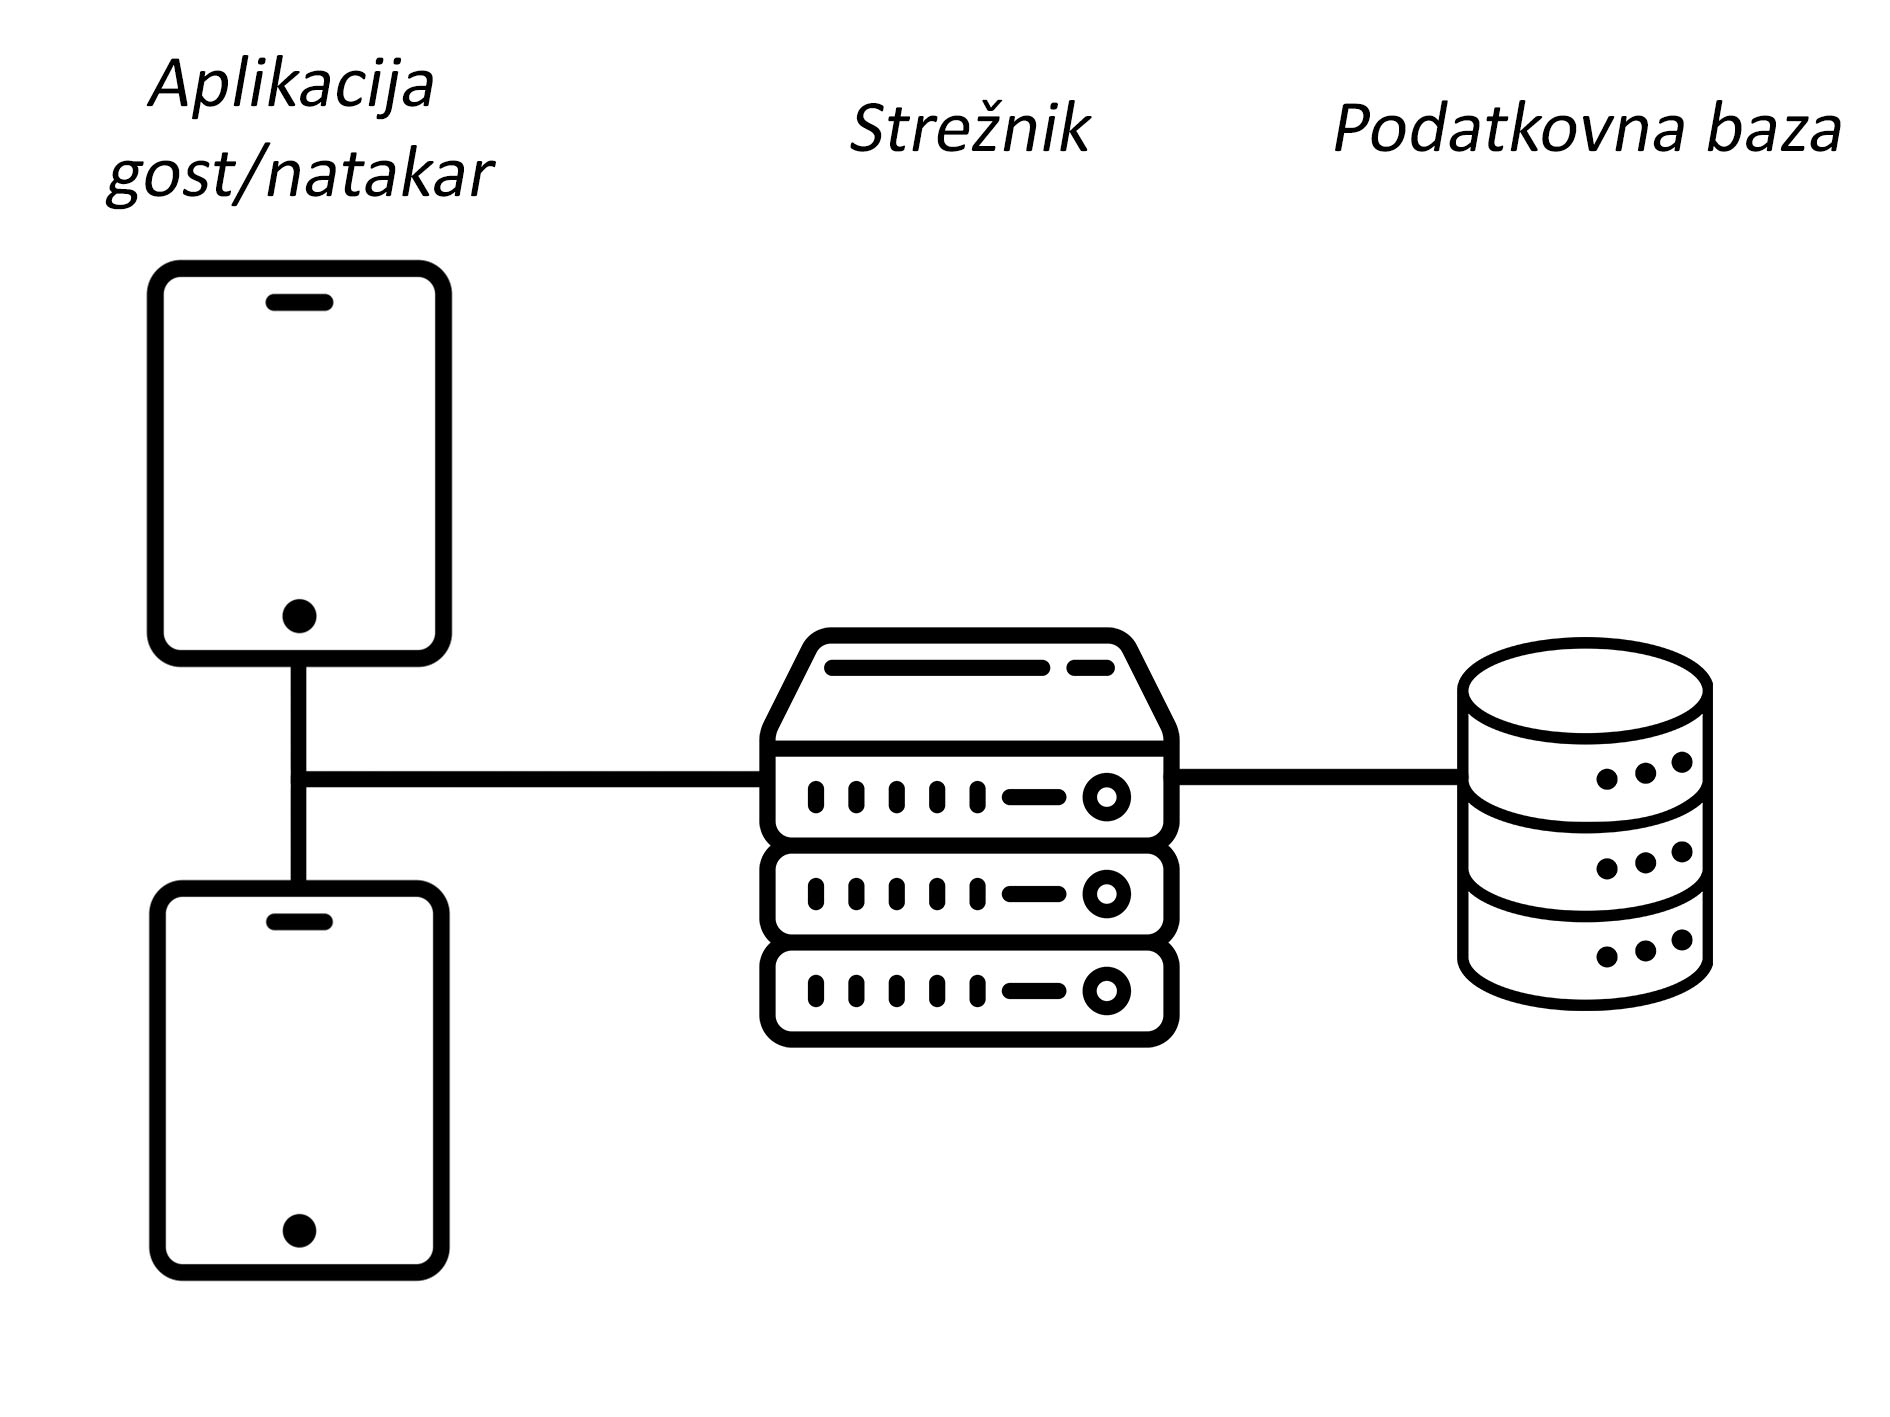
\includegraphics[width=11cm]{Skica1.jpg}
\caption{Struktura aplikacije}
\label{StrukApk}
\end{figure}

Podatkovna baza je namenjena shranjevanju vseh podatkov, ki so pomembni, da se ne izgubijo oziroma se razlikujejo za vsako restavracijo. 
Strežnik je kot neke vrste RESTful vmesnik, ki servira podatke iz podatkovne baze odjemalcu. 
Odjemaleca sta v našem primeru dve ločeni spletni aplikaciji, in sicer za gosta ter natakarja oziroma kuharja, ki je skupen.

Gost lahko odda, spremeni ali zaključi naročilo. Za eno mizo je lahko hkrati odprto eno naročilo. To pomeni, da morajo za mizo naročati skupaj. V restavraciji je lahko večje število miz.
Natakar lahko sprejme, zavrne, uredi ali zaključi naročilo. V restavraciji je lahko večje število natakarjev, ki streže istočasno. 
Kuhar lahko sprejeme, zavrne ali sporoči, da jed za neko naročilo že pripravljena. Restavracija ima lahko več kuharjev, vendar samo en kuhar hkrati lahko uporablja aplikacijo. Omejitev je v podatkovnem modelu.

\begin{figure}[!htb]
\begin{center}
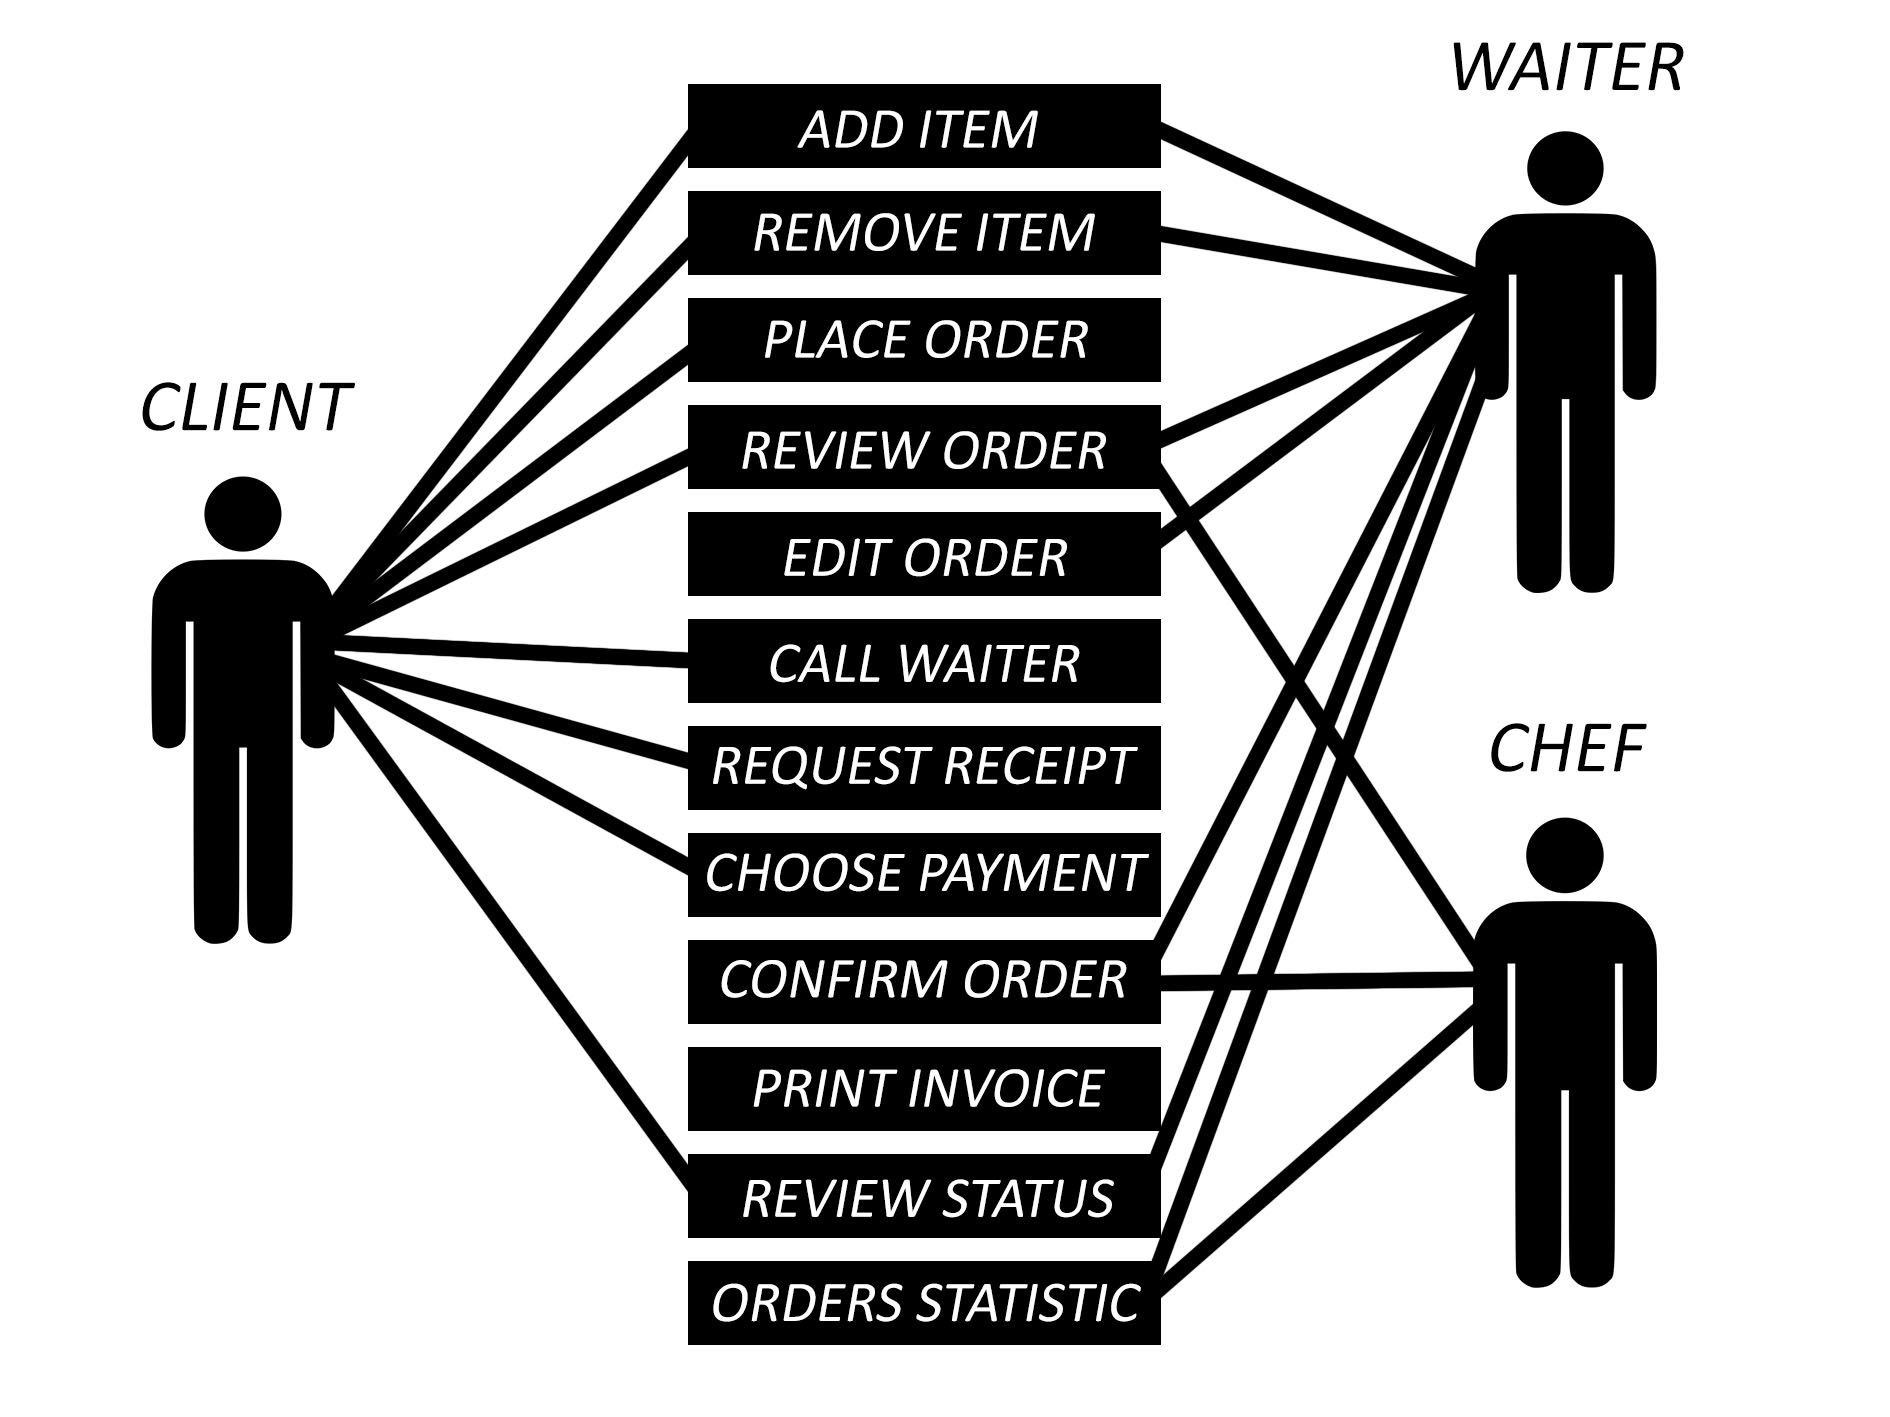
\includegraphics[width=11cm]{Skica2.jpg}
\end{center}
\caption{Diagram primerov uporabe spretnega naročanja}
\label{FunkVloge}
\end{figure}

 

\section{Podatkovna baza}
Na podlagi izdelanega diagrama zahtev oziroma fukcij smo izdelali fizično obliko podatkovne baze (slika~\ref{Database_physical}), katero smo kasneje pretvorili v MySQL. Podatkovna baza je sestavljena je iz šestih tabel, ki so: \textit{ProductType, Product, ProductOrder, Order, User, Table}. 

\begin{figure}[!htb]
\begin{center}
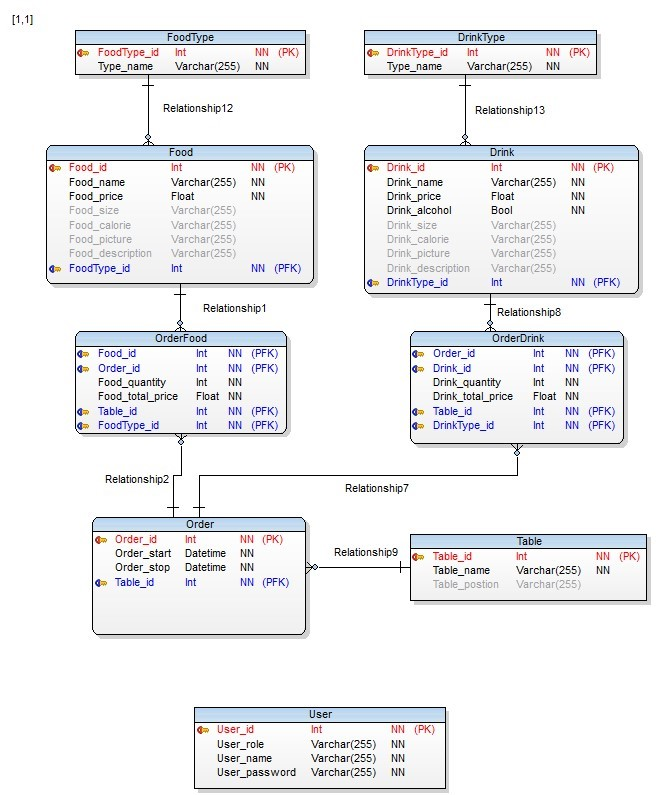
\includegraphics[width=0.85\textwidth]{Database_physical}
\end{center}
\caption{Fizična oblika podatkovne baze}
\label{Database_physical}
\end{figure}

\textit{ProductType} tabela je namenjana zapisom vrsti jedi t.i. predjedi, glavne jedi, sokovi, piva,… Sestavljena je iz atributov ID, Name in Type. Atribut Type je namenjen razlikovanju hrane in pijače. To nam je pomagalo pri razločevanju artiklov v naročilu, saj kuhar ne potrebuje pregleda nad naročili, ki vsebujejo samo pijače. 

\textit{Product} tabela je namenjena opisu hrane in pijače ter je sestavljena iz atributov: ID, Name, Price, Size, Calorie, Picture in Description.  V atribut Picture se zapiše ime slike, ki se prikaže v aplikaciji. Vse slike smo shranjevali v datoteki na lokalnem strežniku Apache.

\textit{ProductOrder} tabela je namenjena količini in končni ceni vsake hrane in pijače v naročilu. Sestavljena je iz atributov: TotalPrice in Quantity. Zapis ne more obstajati če nima definiranega naročila. Tabela je nastala zaradi razmerja M:N t.i. mnogo-proti-mnogo med tabelo Product in Order.

\textit{Order} tabela je namenjena zapisovanju naročila in njegovih podrobnosti. Sestavljena je iz atributov: ID, Start, End, OrderStatus, CookStatus, Payment. Vsebuje tudi tuji ključ ID od table Table, ki je zelo pomemben saj določuje na katero mizo je vezano naročilo. Atributa OrderStatus in CookStatus sta nemanjena sporočanju statusa naročila med vlogami. Uporabil sem ENUM za vrsto parametra, saj gre za vrednosti, ki se ne spreminjajo.

\textit{Table} tabela je namenjena shranjevanju miz v restavracijah. Sestavljajo jo atributi: ID, Name in Position, v katerega se lahko bolj podrobno opiše lokacijo mize.

\textit{User} tabela je namenjena predvsem aplikativnem delu za natakarje in kuharje. Sestavljna je iz atributov: ID, Role, Name in Password. 

Strukturo podatkovne baze smo naredili s pomočjo programa Toad DataModler. To je orodje za izdelavo visokokakovostnih podatkovnih modelov \cite{Toad_Data_Modeler}. Omogoča izdelavo logičnih in fizičnih podatkovnih modelov, kar pripore k lažjem razumevanju in razvijanju podatkovne baze. Njegova najboljša funkcionalnost je, da lahko generiramo SQL kodo v različne podatkovne sisteme kot npr. MySQL, Ingres, Microsoft Azurem, Microsoft Access, Mircrosoft SQL Server,... 

Za izvoz podatkovne baze smo uporabili MySQL. To je eden od odprtokodnih sistemov za upravljanje s podatkovni bazami, ki za delo s podatki uporablja jezik SQL \cite{MySQL}. Napisan je v programskem jeziku C in C++ in deluje v vseh modernih sistemih npr. Windows, Linux, OS X,… Prva verzija je bil razvita leta 1995 s strani Michael Widenius in David Axmark. Kratica My izhaja iz imena prve hčerke očeta Michaela.  

Najbolj zahtevno je bilo napolniti podatkovno bazo, katero delo smo si olajšali s pomočjo phpMyAdmin. To je ime za spletni vmesnik, ki omogoča upravljane z MySQL podatkovnimi bazami. Program je vključen v XAMPP in sicer znotraj aplikacije MySQL. Je zelo močno orodje in predvsem enostavno za uporabo.

\section{Strežnik}
Strežniški del aplikacije smo izdelali po zahtevah RESTful arhitekture, ki vsebuje 6 načel. 

1.)\textit{ Client-server} - zahteva ločitev odjemalca od strežnika kar onemogča odjemalcu direktno povezljivost s podatkovno bazo in s tem poenostavi razširljivost uporabniškega dela. Strežnik ne zanima uporabniški vmesnik ali podatki, tako da je bolj enostaven in prilagodljiv za uporabo. Tako se lahko uporabniški kot strežiški del razvijaj ali zamenjujeje neodvisno.

2.) Stateless - vsaka zahteva od odjemalca mora vsebovati vse potrebne podatke, da pridobi odogovor. Strežnik ne shranjuje lokalno nobenih podatkov od odjemalca, vendar jih glede na zahtevek samo prebere ali pa zapiše v podatkovno bazo.

3.) Cachable - vsak odgovor od strežnika more biti označen kot cacheable or non-cacheable. S tem odjemalec ne zahteva od strežnika eno in isto zadevo, razen če v primeru, da je prišlo do sprememb v podatkih.

4.) Uniform interface - zahteva enoten vmensika API med strežnikom in odjemalcem za določene vire, ki imajo lahko samo en logični URI. Arhitertura omogoča, da se vsak del razvija neodvisno. Zato so tukaj še štiri podnačela, ki vodijo do enotnega vmesnika. kar pomeni da morajo uporabljeni morajo biti standardi oziroma globalni koncepti npr. HTTP standart za opis komunikacije -  - ali gre za GET, POST,...  Mi smo to zagotovili s serviranjem podatkov odjemalcu v JSON formata, ki ga je mogoče uporabiti v vseh programskih jezikih.

5.) Layered system - slojevit sistem, sestavljen iz hierarhičnih slovej z namenom omejevanja komponent.

6.) Code on demand (optional) -  opcijsko načelo. Strežnik na zahtevo odjemalca pošlje oziroma izvede programsko kodo na strani odjemalca.

Vsa zgoraj našteta navodila smo morali upoštevati pri izdelavi strežnika. Tako smo dobili vmesnik, ki na zahtevo odjemalca servira podatke v JSON formatu. Primer na sliki~\ref{ServerEX}, ko odjemalec zahteva podatke vseh pijač iz podatkovne baze (HTTP metoda GET). Strežnik omogoča tudi urejanje in brisanje podatkov v podatkovni bazi, vendar zato more biti ustrezna HTTP metoda POST. Spremljanje zahtevkov, ki prihajajo na strežnik, je mogoče preko CLI vmesnika, slika ~\ref{ServerEX2}, ki v primeru nepopolnosti servirajo ustrezno napako.

\begin{figure}
\begin{center}
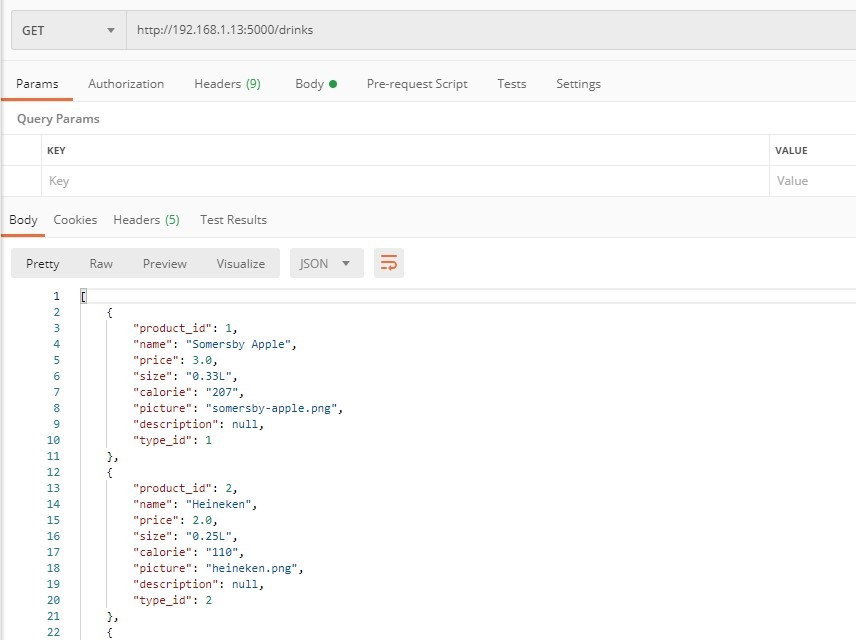
\includegraphics[width=11cm]{Server_example.jpg}
\end{center}
\caption{Primer serviranja podatkov na strežniku}
\label{ServerEX}
\end{figure}
\begin{figure}
\begin{center}
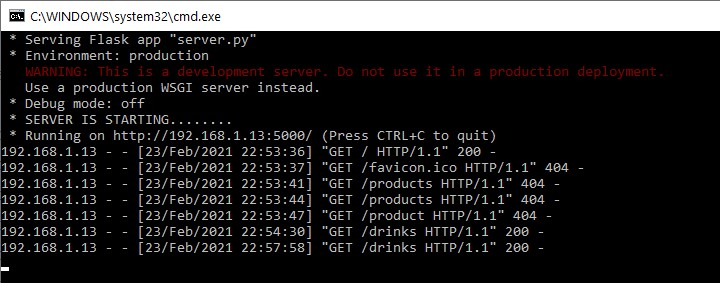
\includegraphics[width=10cm]{Server_example_2.jpg}
\end{center}
\caption{Primer spremljanja zahtevkov, ki prihajajo na strežnik}
\label{ServerEX2}
\end{figure}

Strežnik smo napisali v programske jeziku Python in knjižnici Flask. Zaradi težav s sinhronizacijo podatkov v realnem času na strani odjemalca smo znotraj Flask uporabil še WebSocket. To je napredna tehnologija, ki omogoča odpiranje dvosmerne interaktivne komunikacijske seje med odjemalcem in strežnikom. Primer uporabe je npr. pogovor preko družbenih omrežjih. V naši aplikaciji so s tem lahko vsi odjemalci hkrati obveščani o spremembah na strani podatkovne baze. 

Flask je eno izmed najbolj popularnih spletno aplikacijskih vmesnikov (angl. Freamwork) \cite{Flask}. Zasnovan je tako, da omogoča hiter in enostaven začetek z možnostjo razširitve na zapletene aplikacije. V primerjavi z Django spletnim vmesnikov je za enak primer veliko bolj ekspliciten. Flask je prvotno zasnoval in razvil Armin Ronacher kot prvoaprilsko šalo leta 2010. Kljub taki predstavitvi je Flask postal izjemno priljubljen kot alternativa projektom narejenih v Django. 


Zahtevek:

\begin{verbatim}
C:\Users\lukah>curl -I http://192.168.1.13:5000/drinks
HTTP/1.0 200 OK
Content-Type: application/json
Content-Length: 5066
Access-Control-Allow-Origin: *
Server: Werkzeug/0.16.0 Python/3.7.3
Date: Tue, 02 Mar 2021 20:23:57 GMT
\end{verbatim}

\begin{verbatim}
C:\Users\lukah>curl http://192.168.1.13:5000/drinks 
  {
    "product_id": 1,
    "name": "Somersby Apple",
    "price": 3,
    "size": "0.33L",
    "calorie": "207",
    "picture": "somersby-apple.png",
    "description": null,
    "type_id": 1
  },
  {
    "product_id": 2,
    "name": "Heineken",
    "price": 2,
    "size": "0.25L",
    "calorie": "110",
    "picture": "heineken.png",
    "description": null,
    "type_id": 2
  },
  {
    "product_id": 3,
    "name": "Heineken",
    "price": 3.5,
    "size": "0.5L",
    "calorie": "220",
    "picture": "heineken.png",
    "description": null,
    "type_id": 2
  },
\end{verbatim}

\section{Odjemalec}

Odjemlaca bi načeloma lahko implementirali v spletnih tehnologijah (HTML, CSS, JS) ali pa v namenski mobilni aplikaciji. Mi smo se odločili za programskem jezik JavaScript in knjižnico Vue.  Naredili smo odziven in reaktiven vmesnik, ki deluje v realnem času. Vue je eden izmed mnogih kot npr. Angular, Ember, React,… poznan pa je predvsem zaradi enostavnosti za upravljanje in izvajanje testov. Vsem je skupna točka reaktivnost, vendar v drugačnem pomenu besede. Gre za to, da se aplikacija postopno prilagaja glede na vrednosti podatkov. To prednost sem izkoristil in dodal še knjižnico Vuex, ki služi kot centralizirana baza podatkov za vse komponente v aplikaciji. Podatke i

Da bi to dosegli ne bi potreboali JavaScript zaradi RESTful arhitekutre, ki omogoča katerokoli platformo na strani odjemalca.

\subsection {Kaj je reaktivnost?}
Reaktivnost \cite{reaktivnost}, je programska paradigma, ki nam omogoča, da se na deklarativni način prilagodimo spremembam. Dober primer reaktivnosti je npr. funkcija SUM, ki jo uporabljamo v Excelu. Slika~\ref{Excel-SUM} prikazuje primer v Excelu.
\begin{figure}[h]
\begin{center}
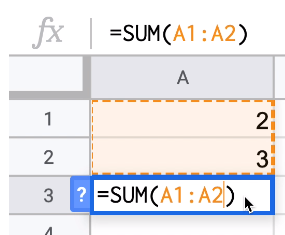
\includegraphics[width=7cm]{Excel-SUM.png}
\end{center}
\caption{Primer fukcije SUM v programu Excel}
\label{Excel-SUM}
\end{figure}

Če vstavimo številko 2 v prvo celico in številko 3 v drugo celico ter izberemo funkcijo SUM teh dveh celic. Kot rezultat dobimo vsoto obeh številk skupaj, kar ni nič posebnega. Vendar če bomo spremenili vrednost prve celice, bo funkcija SUM avtomatsko posodobila skupno vrednost. Tako deluje tudi reaktivnost v aplikacijah za razliko, da je podatek lahko vezan na več funkciji oziroma delov programske kode, ki se ob spremembi vrednosti posodobijo.

\subsection {Delovanje reaktivnost v Vue}
Vue se torej v primerjavi z navadnim JavaScriptom sprehodi skozi podatke in njihove lastnosti (angl. Properties) pretvori v fukciji Getter in Setter, ki sta nevidni uporabniku \cite{delovanjeReaktivnost}. Poglejte si sliko~\ref{VueReacitivity} za lažjo predstavo. 

Torej funkcija Getter pokliče instanco Watcher z namenom odvisnosti do drugih komponent. To pomeni, če je podatek označen kot odvisen (angl.  Dependency) bodo nekateri deli programske kode oziroma funkcije poklicane vsakič, ko se spremeni vrednost podatka. Funkcija Setter pa obvesti instanco Watcher, vsakič ko se podatku spremeni lastnost. Ta poskrbi, da se pokliče funkcija upodabljanja (angl. Render) tiste komponente, ki potem prikaže spremembe v samem pogledu aplikacije. 

\begin{figure}[h]
\begin{center}
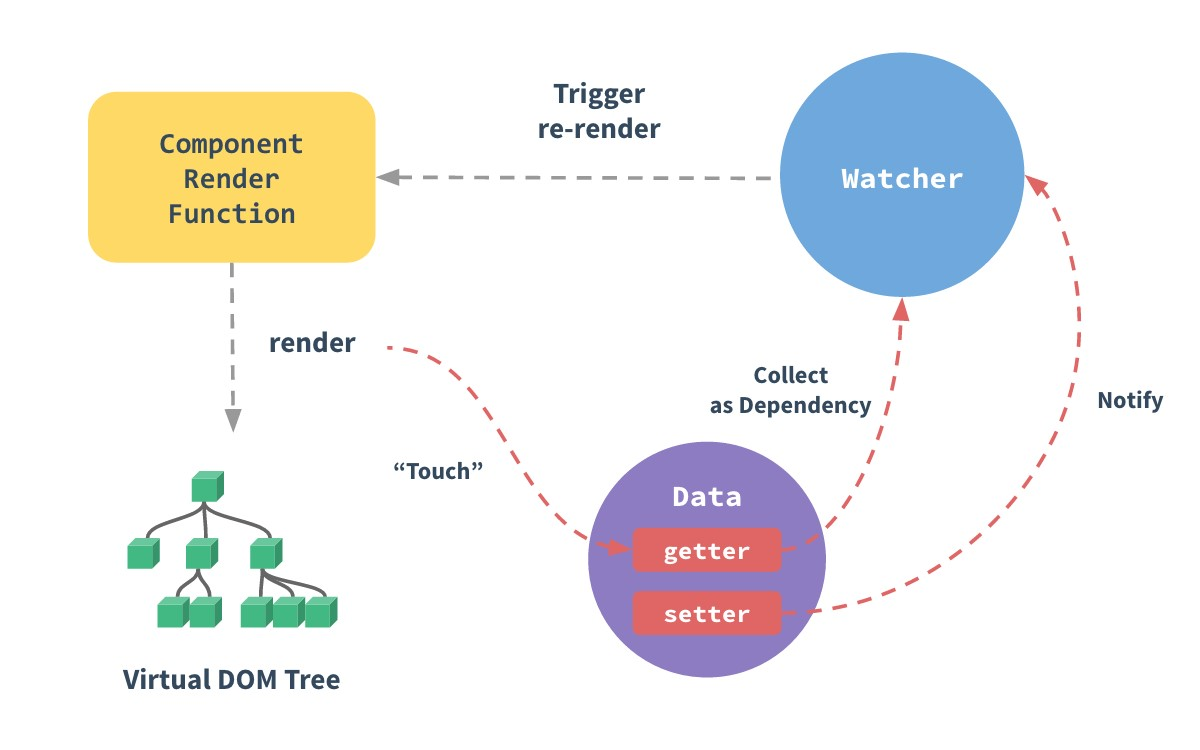
\includegraphics[width=13cm]{Vue-reactivity.jpg}
\end{center}
\caption{Kateri dialekt uporabljati?}
\label{VueReacitivity}
\end{figure}

\subsection {Knjižnice in dodatki}

Tako kot vsak programski jezik ima tudi Vue svoje dodatke, ki pomagajo pri razvoju aplikaciji. Spodnje smo uporabljali in so vredni omembe.
\begin{description}
\item[Vue CLI] velja kot standardno orodje za ekosistem Vue \cite{VueCLI}. Zagotavlja, da že pri gradnji novega projekta poveže različne dodatke med seboj. To omogoča razviljacu, da se bolj osredotoči na programiranje in ne na povezovanje njih v projekt. Zadeva izgleda nekako tako, da preko CLI vmesnika izbereš kakšen projekt želiš. Imaš seveda že privzete nastavitve, vendar omogoča tudi nastavljanje po meri. Sam sem uporabil Vuex, Vue-Router, ESLint in Vuetify.
\item[Vuex] je knjižnica za shranjevanje vrednosti v aplikacijah Vue.js \cite{Vuex}. Služi kot centralizirana baza podatkov za vse komponente v aplikaciji. 
\item[Vue-Router] je uradni usmerjevalnik za Vue.js \cite{VueRouter}. Integrira se globoko z jedrom Vue.js, tako da poenostavi izdelavo SPA aplikacij. Usmerjevalki je mišljen v smislu usmerjanja na druge komponente (angl. Component), ki v Vue.js predstavljajo druge poglede, lahko bi rekli podobno kot podstrani.
\item[ESLint] je orodje za prepoznavanje in poročanje o popravkih v programski kodi \cite{ESLint}. Cilje je narediti kodo bolj pregledno in urejeno, kar pripomore k izogibanju napak.
\item[Vuetify] je eden izmed mnogih uporabniških vmesnikov, ki je zgrajen na vrhu Vue.js \cite{Vuetify}. Za razliko od drugih vmesnikov je Vuetiy enostaven za učenje z več stotimi komponentami izdelanih po specifikacijah Material Design.
\item[Vue-devtools] je zgolj dodatek v brskalniku, ki omogoča lažje sledenje delovanja aplikacije in odpravljanju napak. 
\end{description}


\chapter {Delovanje aplikacije}
\section{Vmesnik za gosat}
\section{Vmesnik za natakarja}
\section{Vmesnik za kuharja}

\chapter {Diskusija}

\chapter {Sklepne ugotovitve}
\newpage %dodaj po potrebi, da bo številka strani za Literaturo v Kazalu pravilna!
\ \\
\clearpage
\addcontentsline{toc}{chapter}{Literatura}
\bibliographystyle{plain}
\bibliography{literatura}


\end{document}

